\subsection{Login}
\label{sub:login}

Det første modul der interageres med, er loginmodulet, som har til formål at validere, og videresende brugeren til programmets hovedfunktioner.

\subsubsection{Funktionalitet}
\label{ssub:login_funktionalitet}

Loginmodulet har det primære ansvar for at angive adgangsniveauer, og sikre databeskyttelse. Fra loginmodulet kan man vælge at oprette sig som ny gæst, eller logge ind i systemet. Hvis brugeren vælger at oprette sig som ny gæst, så vil brugeren blive sendt til et separat modul.

\subsubsection{Implementation}
\label{ssub:login_implementation}

\begin{figure}
  \centering
  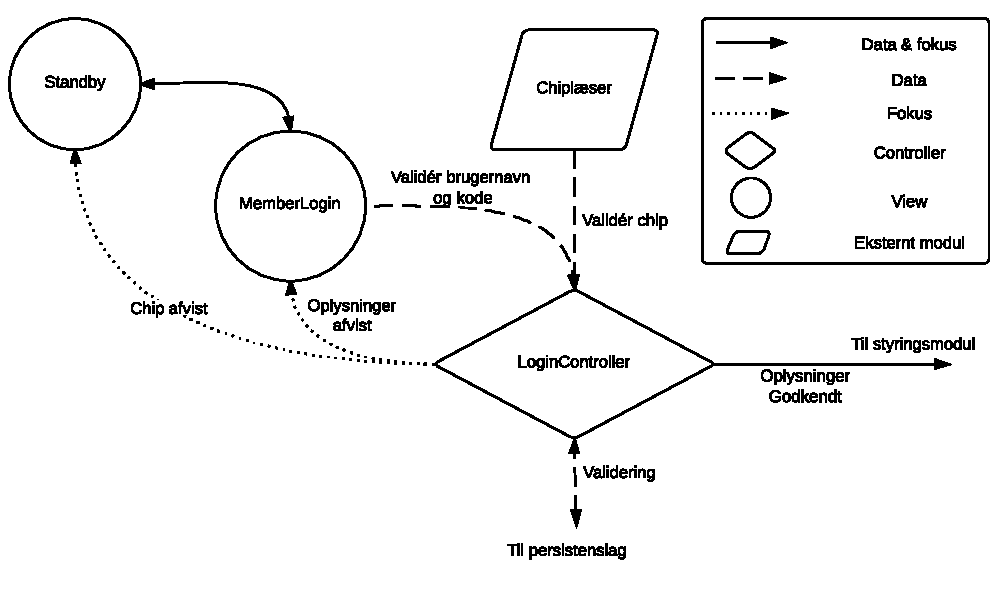
\includegraphics[width=\textwidth]{login-diagram.pdf}
  \caption{Diagram over Loginmodul}
\end{figure}

Loginmodulet består af et standby-view, et MemberLogin-view, et eksternt chiplæsermodul samt en loginController. Fra standby view er der adgang til GuestCreatormodulet, som er beskrevet i \cref{sub:GuestCreator}. Brugeren kan også indlæses et chip-kort, eller skifte til MemberLogin-view. Fra MemberLogin-view, kan der indtastes medlemsnummer og kode.

LoginControlleren modtager data fra memberLogin-view, eller chiplæser-modulet. Denne data valideres, via persistenslaget, i forhold til databasens data. Hvis der ikke kan gennemføres en succesfuld validering, sender loginControlleren brugeren tilbage til det view, der blev sendt data fra, hvor brugeren promptes for nyt indput.

Hvis valideringen er succesfuld, sendes brugeren samt brugerens data, videre til funktionsstyringsmodulet.
